\documentclass[12pt]{ximera}
\title{Homework 4: Introduction to Probability}
\begin{document}
\begin{abstract}
Section 7.3: sample spaces and whether their outcomes are equally likely,
inclusion-exclusion applied to probabilities, and a three-set Venn diagram of blood
antigen frequencies.
\end{abstract}
\maketitle

\section*{Section 7.3: Introduction to Probability}

\begin{problem}
Suppose we run an experiment where each trial consists of flipping a coin three
times. Let $H$ denote heads and $T$ denote tails.

\begin{prompt}
\textbf{(a)} What is the sample space for this experiment if all we want to record
is how many heads are flipped in each trial?

The sample space has $\answer{4}$ outcomes. Listed in increasing order, they are
$\set{\answer{0},\ \answer{1},\ \answer{2},\ \answer{3}}$.

\begin{feedback}
If we record only the \emph{number} of heads, the possible results are
$0$, $1$, $2$, or $3$ heads, so the sample space is $\set{0,1,2,3}$ --- four
outcomes.
\end{feedback}
\end{prompt}

\begin{prompt}
\textbf{(b)} What is the sample space for the experiment if we also want to record
the order of heads and tails flipped?

This sample space has $\answer{8}$ outcomes.

\begin{hint}
Each of the three flips independently has $2$ possible results.
\end{hint}

\begin{feedback}
Recording order, the sample space is
\[
\set{HHH,\ HHT,\ HTH,\ THH,\ HTT,\ THT,\ TTH,\ TTT},
\]
which has $2^3=8$ outcomes.
\end{feedback}
\end{prompt}

\begin{prompt}
\textbf{(c)} Are the probabilities of the outcomes in part (a) all equal?

\begin{multipleChoice}
\choice{Yes --- there are four outcomes, so each has probability $\frac14$}
\choice[correct]{No --- some counts of heads arise from more ordered outcomes than others}
\end{multipleChoice}

\begin{feedback}
No. The eight \emph{ordered} outcomes in part (b) are equally likely, each with
probability $\frac18$, but they are not spread evenly over the four counts:
\[
P(0)=\tfrac18,\quad P(1)=\tfrac38,\quad P(2)=\tfrac38,\quad P(3)=\tfrac18,
\]
because $1$ head happens in three ways ($HTT$, $THT$, $TTH$) while $0$ heads happens
in only one way ($TTT$).

This is the key lesson: ``there are $4$ outcomes'' does not by itself mean each has
probability $\frac14$. The outcomes must be equally likely first.
\end{feedback}
\end{prompt}
\end{problem}

\begin{problem}
Suppose the weather report predicts that there is a $40\%$ chance of rain and a
$35\%$ chance of high winds, with a $15\%$ chance of both. Use inclusion-exclusion
or a Venn diagram to answer the following.

\begin{prompt}
\textbf{(a)} What is the probability that there will be rain or high winds (or
both)?

$\answer[tolerance=0.001]{0.6}$

\begin{hint}
$P(R\cup W)=P(R)+P(W)-P(R\cap W)$. Enter your answer as a decimal.
\end{hint}

\begin{feedback}
\[
P(R\cup W)=P(R)+P(W)-P(R\cap W)=0.40+0.35-0.15=0.60,
\]
so there is a $60\%$ chance of rain or high winds (or both).
\end{feedback}
\end{prompt}

\begin{prompt}
\textbf{(b)} What is the probability that there will be no rain and no high winds?

$\answer[tolerance=0.001]{0.4}$

\begin{hint}
``No rain and no wind'' is the complement of ``rain or wind''.
\end{hint}

\begin{feedback}
``Neither'' is the complement of ``either'', so
\[
P\left(\olsi{R}\cap\olsi{W}\right)=1-P(R\cup W)=1-0.60=0.40,
\]
a $40\%$ chance.
\end{feedback}
\end{prompt}
\end{problem}

\begin{problem}
On their surface, red blood cells have inherited chemical structures called antigens
that can cause a person's immune system to make antibodies against them. Every human
has a particular combination of antigens on the surface of their blood cells, and
their immune system will create antibodies against any antigens that are not among
their own.

There are many major and minor groups of these antigens, but in particular,
consideration of the presence of A, B, and Rh antigens is necessary to ensure that a
transfusion recipient receives compatible blood.

For example, someone with A antigens but neither B nor Rh antigens (commonly called
``A-negative'' or ``A$-$'' blood type) could donate blood to anyone who has A
antigens (that is, anyone with A$+$, A$-$, AB$+$, or AB$-$ blood type), but could
only receive a transfusion from someone with neither B nor Rh antigens (that is,
anyone with A$-$ or O$-$ blood type, where ``O'' signifies the absence of A or B
antigens).

The following data about blood type frequency was reported by the National Health
Service in 2018. Among blood donors,
\begin{itemize}
    \item $75\%$ have Rh antigens;
    \item $41\%$ have A antigens;
    \item $13\%$ have B antigens;
    \item $32\%$ have Rh and A antigens;
    \item $10\%$ have Rh and B antigens;
    \item $3\%$ have A and B antigens;
    \item $2\%$ have all three of these antigens.
\end{itemize}

\begin{prompt}
\textbf{(a)} Fill in the seven regions of the Venn diagram, as percentages. Work
from the center outward.

\begin{center}
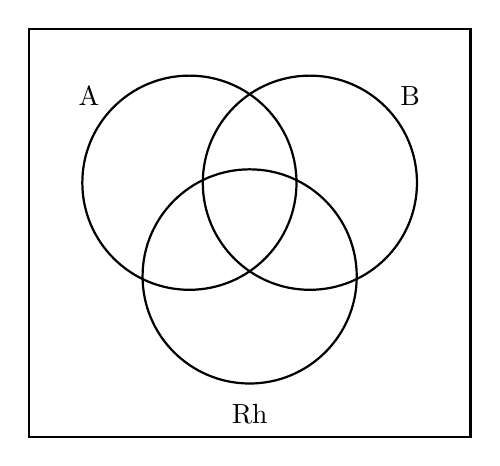
\begin{tikzpicture}[scale=0.85]
  \draw[thick] (-0.9,0.5) circle (1.6) node at (-2.4,1.8) {A};
  \draw[thick] (0.9,0.5) circle (1.6) node at (2.4,1.8) {B};
  \draw[thick] (0,-0.9) circle (1.6) node at (0,-2.95) {Rh};
  \draw[thick] (-3.3,-3.3) rectangle (3.3,2.8);
\end{tikzpicture}
\end{center}

All three antigens (the center): $\answer{2}\%$

\smallskip
A and B but not Rh: $\answer{1}\%$ \qquad
A and Rh but not B: $\answer{30}\%$ \qquad
B and Rh but not A: $\answer{8}\%$

\smallskip
A only: $\answer{8}\%$ \qquad
B only: $\answer{2}\%$ \qquad
Rh only: $\answer{35}\%$

\begin{hint}
Start with the center ($2\%$, given directly) and work outward. Each two-antigen
figure, such as the $3\%$ with A and B, \emph{includes} the people who have all
three --- so subtract the center from it to get the ``exactly these two'' region.
\end{hint}

\begin{feedback}
Start at the center and work out.
\begin{itemize}
\item All three: $2\%$, given.
\item A and B: the $3\%$ includes the $2\%$ with all three, so A and B but not Rh is
      $3-2=1\%$.
\item A and Rh: $32-2=30\%$.
\item B and Rh: $10-2=8\%$.
\item A only: the whole A circle is $41\%$, from which we remove the three regions
      just found that sit inside it: $41-(1+30+2)=8\%$.
\item B only: $13-(1+8+2)=2\%$.
\item Rh only: $75-(30+8+2)=35\%$.
\end{itemize}
\end{feedback}
\end{prompt}

\begin{prompt}
\textbf{(b)} What is the probability that a donor's blood contains none of these
antigens (O$-$)?

$\answer{14}\%$

\begin{hint}
Add up all seven regions inside the circles and subtract from $100\%$.
\end{hint}

\begin{feedback}
The seven regions inside the diagram total
\[ 2+1+30+8+8+2+35 = 86\%, \]
so the region outside all three circles is $100-86=14\%$.
\end{feedback}
\end{prompt}

\begin{prompt}
\textbf{(c)} Per the example above, what is the probability a random donor's blood
type is compatible as a transfusion for someone with A antigens but neither B nor Rh
antigens (A$-$)?

$\answer{22}\%$

\begin{hint}
Re-read the example: an A$-$ recipient can accept blood only from A$-$ or O$-$
donors. Which two regions of your diagram are those?
\end{hint}

\begin{feedback}
An A$-$ recipient can receive blood only from donors with neither B nor Rh antigens,
which is A$-$ blood (the ``A only'' region) or O$-$ blood (the region outside all
three circles). From parts (a) and (b), those are $8\%$ and $14\%$, so
\[ 8\% + 14\% = 22\%. \]
\end{feedback}
\end{prompt}
\end{problem}

\end{document}
